\documentclass[]{scrartcl}
% Лицензия
% Apache License Version 2.0, January 2004
% http://www.apache.org/licenses/
% Copyright [2020] [Kirill A. Murashev]
% Licensed under the Apache License, Version 2.0 (the "License"); you may not use this file except in compliance with the License. You may obtain a copy of the License at
% http://www.apache.org/licenses/LICENSE-2.0
% Unless required by applicable law or agreed to in writing, software
% distributed under the License is distributed on an "AS IS" BASIS,
% WITHOUT WARRANTIES OR CONDITIONS OF ANY KIND, either express or implied.
% See the License for the specific language governing permissions and limitations under the License.


%%% Работа с русским языком
\usepackage{cmap}					% поиск в PDF
\usepackage{mathtext} 				% русские буквы в формулах
\usepackage{fontspec}
\defaultfontfeatures{Renderer=Basic,Ligatures={TeX}}
\setmainfont{CMU Serif}
\setsansfont{CMU Sans Serif}
\setmonofont{CMU Typewriter Text}
\usepackage[english,russian]{babel}
%\usepackage[T1,T2A]{fontenc}			% кодировка
%\usepackage[lutf8]{luainputenc}			% кодировка исходного текста
%\usepackage[english,russian]{babel}	% локализация и переносы
\usepackage{indentfirst}            % красная строка
\usepackage{misccorr}               % доработки для babel
\frenchspacing                      % французский стиль пробелов

%\usepackage{beton} %изменение шрифта для тёмной цветовой схемы
%\usepackage{concrete}
%%% Дополнительная работа с математикой
\usepackage{amsmath,amsfonts,amssymb,amsthm,mathtools} % AMS
\usepackage{icomma} % "Умная" запятая: $0,2$ --- число, $0, 2$ --- перечисление

%% Номера формул
%\mathtoolsset{showonlyrefs=true} % Показывать номера только у тех формул, на которые есть \eqref{} в тексте.
%\usepackage{leqno} % Нумерация формул слева

%% Перенос знаков в формулах (по Львовскому)
\newcommand*{\hm}[1]{#1\nobreak\discretionary{}
	{\hbox{$\mathsurround=0pt #1$}}{}}

%%% Работа с картинками
\usepackage{graphicx}  % Для вставки рисунков
\graphicspath{{Images/}}  % папки с картинками
\setlength\fboxsep{3pt} % Отступ рамки \fbox{} от рисунка
\setlength\fboxrule{1pt} % Толщина линий рамки \fbox{}
\usepackage{wrapfig} % Обтекание рисунков текстом

%%% Работа с таблицами
\usepackage{array, tabularx, tabulary, booktabs, xtab} % Дополнительная работа с таблицами
\usepackage{longtable}  % Длинные таблицы
\usepackage{multirow} % Слияние строк в таблице

%%% Теоремы
\theoremstyle{plain} % Это стиль по умолчанию, его можно не переопределять.
\newtheorem{theorem}{Теорема}[section]
\newtheorem{proposition}[theorem]{Утверждение}

\theoremstyle{definition} % "Определение"
\newtheorem{corollary}{Следствие}[theorem]
\newtheorem{problem}{Задача}[section]

\theoremstyle{remark} % "Примечание"
\newtheorem*{nonum}{Решение}

%%% Программирование
\usepackage{etoolbox} % логические операторы

\usepackage{lastpage} % Узнать, сколько всего страниц в документе.

\usepackage{keyval}

\usepackage{totcount} % Узнать, сколько всего объектов в документе.

%\usepackage{xcolor-solarized}

%%% Страница
%\usepackage{extsizes} % Возможность сделать 14-й шрифт
%\usepackage{geometry} % Простой способ задавать поля
%	\geometry{top=25mm}
%	\geometry{bottom=35mm}
%	\geometry{left=35mm}
%	\geometry{right=20mm}
%

%\usepackage{fancyhdr} % Колонтитулы

%	\pagestyle{fancy}
%\renewcommand{\headrulewidth}{0pt}  % Толщина линейки, отчеркивающей верхний колонтитул
%\fancyhf{}
%\lhead{Часть \thepart}
%\chead{Глава \thechapter}
%\rhead{Раздел \thesection}
%\lfoot{version 0.251}
%\cfoot{\today} % По умолчанию здесь номер страницы
%\rfoot{\thepage/\ref{LastPage}}
%\pagestyle{fancy}

%\usepackage{setspace} % Интерлиньяж
%\onehalfspacing % Интерлиньяж 1.5
%\doublespacing % Интерлиньяж 2
%\singlespacing % Интерлиньяж 1

\usepackage{soul} % Модификаторы начертания

\usepackage[usenames,dvipsnames,svgnames,table,rgb]{xcolor} % Подключение пакета для задания цвета

%\definecolor{Backcolor}{HTML}{042029} % Задание цвета для фона
%\definecolor{Textcolor}{HTML}{819090} % Задание цвета для текста
%\pagecolor{Backcolor}                 % Подключение тёмной
%\color{Textcolor}                     % темы

\usepackage{csquotes} % Ещё инструменты для ссылок

\usepackage[backend=biber,bibencoding=utf8,sorting=ynt,maxcitenames=5,sortupper=true,date=iso]{biblatex} % подключение пакета для работы с автоматизированной библиографией

%\usepackage[style=authoryear,maxcitenames=2,backend=biber,sorting=nty]{biblatex}

%\renewcommand\bibname{Источники информации} % Переопределение названия для библиографии

\usepackage{multicol} % Несколько колонок

\usepackage{microtype}              %<-- added for better inter word spacing

\usepackage{tabularx}

\usepackage{tikz} % Работа с графикой
\usepackage{pgfplots}
\usepackage{pgfplotstable}

\usepackage{eqlist}

\usepackage{desclist} % Дополнительное окружение для списка Глоссария

\usepackage{lineno} % Нумерация строк

\setcounter{tocdepth}{8} % Глубина оглавления

% подавление висячих строк
\clubpenalty=400 % Разрешение = 300, абсолютный запрет = 10000
\widowpenalty=400 % Увеличиваем эти числа до тех пор, пока не начнёт увеличиваться количество страниц.

% Выбор между разрежением и переполнением
\tolerance=500 % max=10000, default=200

\looseness=-1 % иногда можно удлинять страницу на одну строку.

\hfuzz=2.5pt % иногда можно вылезти за край строки на 2.5 pt.

\usepackage{calc} % Вычисления

\usepackage{scrlayer-scrpage} % Стиль страницы

\usepackage{lineno} % нумерация строк

%\pagestyle{scrpage}

%\usepackage{concrete}

\usepackage{booktabs}

\usepackage[owncaptions]{vhistory} % Log of versions

\usepackage{progressbar} % Формирование линейки, показывающей прогресс в работе

\usepackage{epigraph} % работа с эпиграфами

\usepackage {listings}
\lstloadlanguages{[Latex]Tex, bash, R, Python, SQL}
\lstset{extendedchars=true , % включаем не латиницу
frame=tb, % рамка сверху и снизу
commentstyle=\itshape , % шрифт для комментариев
stringstyle =\ttfamily % шрифт для строк
%keywordstyle=\color{blue}
}

%\usepackage{titling} %дополнительная настройка титульного листа

\setcounter{secnumdepth}{8} % Установка глубины нумерации заголовков

% Работа с гиперрсылками, подключается последним
\usepackage{hyperref}       % Подключение пакета для работы с гиперссылками
\hypersetup{				% Гиперссылки
	unicode=true,           % русские буквы в раздела PDF
	pdftitle={Искусственный интеллект в~оценке стоимости},   % Заголовок
	pdfauthor={К.\,А.~Мурашев},      % Автор
	pdfsubject={Системы поддержки принятия решений, основанные на искусственном интеллекте},      % Тема
	pdfcreator={К.\,А.~Мурашев}, % Создатель
	pdfproducer={К.\,А.~Мурашев}, % Производитель
	pdfkeywords={Искусственный интеллект, машинное обучение, математические методы, оценочная деятельность, цифровая экономика, Data Science, анализ данных} % Ключевые слова
	colorlinks=true,       	% false: ссылки в рамках; true: цветные ссылки
	linkcolor=red,          % внутренние ссылки
	citecolor=green,        % на библиографию
	filecolor=magenta,      % на файлы
	urlcolor=blue           % на URL
}

\usepackage{pgfplots} 
\pgfplotsset{compat=1.15}
\usepackage{mathrsfs}
\usetikzlibrary{arrows}
%\usepackage{url}

%\usepackage{totpages}

%\usepackage[strings]{underscore}

%\author{К.\,А.~Мурашев\thanks {\href{kirill.murashev@tutanota.de}{kirill.murashev@tutanota.de}, \href{https://t.me/Maas\_88}{https://t.me/Maas\_88}, \href{https://www.facebook.com/murashev.kirill}{https://www.facebook.com/murashev.kirill}}}
%\title{\Large Современные системы поддержки принятия решений оценщиками, основанные на~применении методов машинного обучения: практическое руководство по~применению языка программирования R в~повседневной практике оценщика}
%\date{\today}

%\normalsize

% Макрос для рисунков, обтекаемых текстом
\newcommand*{\EpsWrapD}[7]{%
	\begin{wrapfigure}[#5]{#3}{#2 \textwidth} % #3=l,r,L,R
		\begin{center} \sffamily
			\includegraphics*[width= #2 \textwidth ]{#1} % 1-имя файла и метка заодно,
			% 2-ширина рисунка (доля от ширины страницы)
			\vspace{-#7mm} % #7: сократить расстояние между подписью снизу и рисунком
			\caption{\label{fig:#1}#4} % #4 - подпись под рисунком
			\vspace{-#6pt}
		\end{center}% #6: сократить расстояние между подписью снизу и текстом после таблицы 
	\end{wrapfigure}}
%
% макрос для создания таблицы, обтекаемой текстом
\newcommand*{\TableBE}[5]{
	\begin{table}[#1] %\captionabove
		\vspace*{-#5mm}
		\centering \sffamily \caption{\label{tab:#2}#3} \begin{tabular}{#4} \toprule }
		
		\newcommand*{\TableEN}[3]{
			\bottomrule \end{tabular}
		\vspace{-#2mm} \small \begin{flushleft} #1 \end{flushleft}
		\vspace{-#3mm}
\end{table}}


\addbibresource{/home/kaarlahti/TresoritDrive/Methodics/My/AI_for_valuers/Book/AI_for_valuers_book/Basic_principles.bib}
\addbibresource{/home/kaarlahti/TresoritDrive/Methodics/My/AI_for_valuers/Book/AI_for_valuers_book/LaTeX.bib}
\addbibresource{/home/kaarlahti/TresoritDrive/Methodics/My/AI_for_valuers/Book/AI_for_valuers_book/Mathstat.bib}
\addbibresource{/home/kaarlahti/TresoritDrive/Methodics/My/AI_for_valuers/Book/AI_for_valuers_book/Murashev.bib}
\addbibresource{/home/kaarlahti/TresoritDrive/Methodics/My/AI_for_valuers/Book/AI_for_valuers_book/Python.bib}
\addbibresource{/home/kaarlahti/TresoritDrive/Methodics/My/AI_for_valuers/Book/AI_for_valuers_book/R.bib}
\addbibresource{/home/kaarlahti/TresoritDrive/Methodics/My/AI_for_valuers/Book/AI_for_valuers_book/RussianLaws.bib}
\addbibresource{/home/kaarlahti/TresoritDrive/Methodics/My/AI_for_valuers/Book/AI_for_valuers_book/Sci&Tech.bib}
\addbibresource{/home/kaarlahti/TresoritDrive/Methodics/My/AI_for_valuers/Book/AI_for_valuers_book/Valuation.bib}
\addbibresource{/home/kaarlahti/TresoritDrive/Methodics/My/AI_for_valuers/Book/AI_for_valuers_book/ValuationStandards.bib}
\addbibresource{/home/kaarlahti/TresoritDrive/Methodics/My/AI_for_valuers/Book/AI_for_valuers_book/ZHZL.bib}

\pagestyle{headings} 
\markright{Искусственный интеллект в~оценке стоимости}
\usepackage{pgfplots}
\pgfplotsset{compat=1.15}
\usepackage{mathrsfs}
\usetikzlibrary{arrows}

%\usepackage{polyglossia}

%\usepackage{minted}

\newtheorem{Thexmpl}[theorem]{Пример}

\usepackage[inkscapearea=page]{svg}
\usepackage{adjustbox}


\title{Очень краткое введение в~математическую статистику для~оценщиков}
\author{К.\,А.\,Мурашев}

\begin{document}

\maketitle

\begin{abstract}
	Какую~бы работу не~выполнял оценщик, во~всех случаях он~имеет дело с~информацией и~данными. Часто эти~данные представляют собой числа либо могут быть формализованы иным образом. В~любом случае требуется алгоритмическая обработка входных данных и~преобразование их~в~информацию, а~в~некоторых случаях "--- в~знания. Целью данного фрагмента является формирование общих представлений об~основных понятиях и~методах математической статистики, необходимых современному оценщику. Автор постарался прибегать к~минимальному числу формул и~сложных определений, хотя это~и~не~вполне получилось. Поскольку конечной целью всей работы является цифровизация оценочной деятельности, в~тексте приводятся короткие листинги на~языках R и~Python, позволяющие реализовать то, о~чём говорится в~тексте.
\end{abstract}

\section{Что~есть математическая статистика?}
У~термина <<статистика>> существует несколько определений. Статистикой называют:
	\begin{itemize}
		\item данные, количественно описывающие тот~или~иной аспект окружающего мира: например данные об~уровне безработицы, заболеваемости коронавирусом или~доходах граждан, т.\,е.~такие данные, которые описывают явление целиком;
		\item количественные данные, относящиеся к~какому-либо одному субъекту либо результатам его~деятельности: например количество выполненных оценщиком отчётов об~оценке за~календарный год;
		\item результаты исследования отдельных выборок: например итоги социологических опросов или~результаты анализа рынка недвижимого имущества;
		\item конкретные методы анализа данных с~помощью математичсеских методов;
		\item т.\,н. статистики критерия, т.\,е.~конкретные числовые значения отдельных вычислений, например статистика критерия Шапиро"--~Уилка;
		\item область знаний, которая разрабатывает и~использует математические методы для~описания данных и~формирования суждений о~них.		   
	\end{itemize}

\textbf{Первый} тип статистики как правило не~имеет прямого отношения к~деятельности оценщика. Подобные сведения чаще всего могут быть получены из~открытых источников. Кроме того, даже в~случае недоверия к~ним, у~оценщика всё~равно отсутствуют инструменты для~получения подобных данных самостоятельно. \textbf{Второй} тип "--- скорее всего также не~является особенным предметом интереса оценщика. Определение стоимости объекта осуществляется методом аналогии путём сравнения с~наблюдениями~(предложениями либо сделками), тогда как~погружение в~свойства только самого объекта не~позволяют определить его~стоимость. \textbf{Третий} тип статистики отсылает нас~к~фундаментальному принципу: исследовать генеральную совокупность путём изучения выборки из~неё. Собственно это~и~является предметом данной работы, а~также профессиональной деятельности оценщика: формирование предсказания свойства объекта (его~стоимости) на~основе изучения выборки. \textbf{Четвёртый} "--- является ключевым с~узко практической точки зрения. Процесс предсказывания неизвестных свойств объектов на~основе известных с~учётом знаний, полученных при~изучении выборки, по~мнению многих, и~есть статистика. Данный подход не~является ошибочным, однако его~вряд~ли можно считать полным. Умение применять конкретные методы является необходимым, но~недостаточным условием успешной работы. В~настоящее время практически все~вычисления выполняются программными средствами.\footnote{Автор в~своей работе использует языки программирования Python и~R и~рекомендует поступать также, однако существуют и~иные средства: Julia, SPSS, PSPP, Stata и~многие другие вплоть до~табличных процессоров.} В~связи с~этим важность навыков ручного применения тех~или~иных методов сведена к~минимуму. Вместо этого на~первый план выходят навыки планирования оценочного статистического эксперимента, постановки задачи, поиск источников данных, их~сбор и~предобработка, общее понимание применяемых методов, выбор между ними, а~также интерпретация полученного результата. \textbf{Пятый} тип означает результаты применения конкретных методов. В~настоящее время чаще используются не~сами статистики критериев, а~универсальный показатель "--- p-значение~(p-value). И, наконец, \textbf{шестое} определение означает обширную область человеческих знаний, в~рамках которой существуют конкретные методы и~результаты их~применения. Данное определение может быть заменено термином \emph{<<математическая статистика>>}, подчёркивающим отличие от~других значений общего термина <<статистика>>. Именно в~этом значении мы~и~будем использовать данный термин на~протяжении всей работы по~ознакомлению со~статистическими основами оценки стоимости. Таким образом, если в~тексте прямо не~указано иное слово <<статистика>> следует понимать как~<<математическая статистика>>.

\section{Генеральная совокупность и~выборка}
Генеральной совокупностью называется всё~множество объектов, в~отношении которого необходимо сделать те~или~иные выводы. В~случае оценки, например торгово-развлекательного центра, расположенного на~проспекте Просвещения в~Санкт-Петербурге, генеральной совокупностью будут являться все~торговые центры, расположенные на~территории Санкт-Петербургской городской агломерации, независимо от~того, выставлены они~в~данный момент на~продажу или~нет. Для~того, чтобы понять, что~является генеральной совокупностью, необходимо ответить на~один простой вопрос: <<на~какое множество объектов можно обобщить полученные результаты исследования?>>. Очевидно, что~независимо от~того, выставлен~ли какой-либо из~существующих в~агломерации ТРЦ на~продажу или~нет, совершались~ли с~ним в~последнее время сделки или~нет, все~выводы, сделанные относительно множества <<торгово-развлекательные центры, расположенные в~СПБГА,\footnote{Санкт-Петербургская городская агломерация. Включает в~себя Санкт-Петербург, б\'ольшую часть Всеволожского, части Выборгского, Кировского, Тосненского, Гатчинского и~Ломоносовского районов Ленинградской области.} могут быть распространены на~него равно как~и~на~вообще любой объект данного типа, находящийся в~указанных границах.
 
\begin{figure}[ht]
\centering % Центрируем картинку
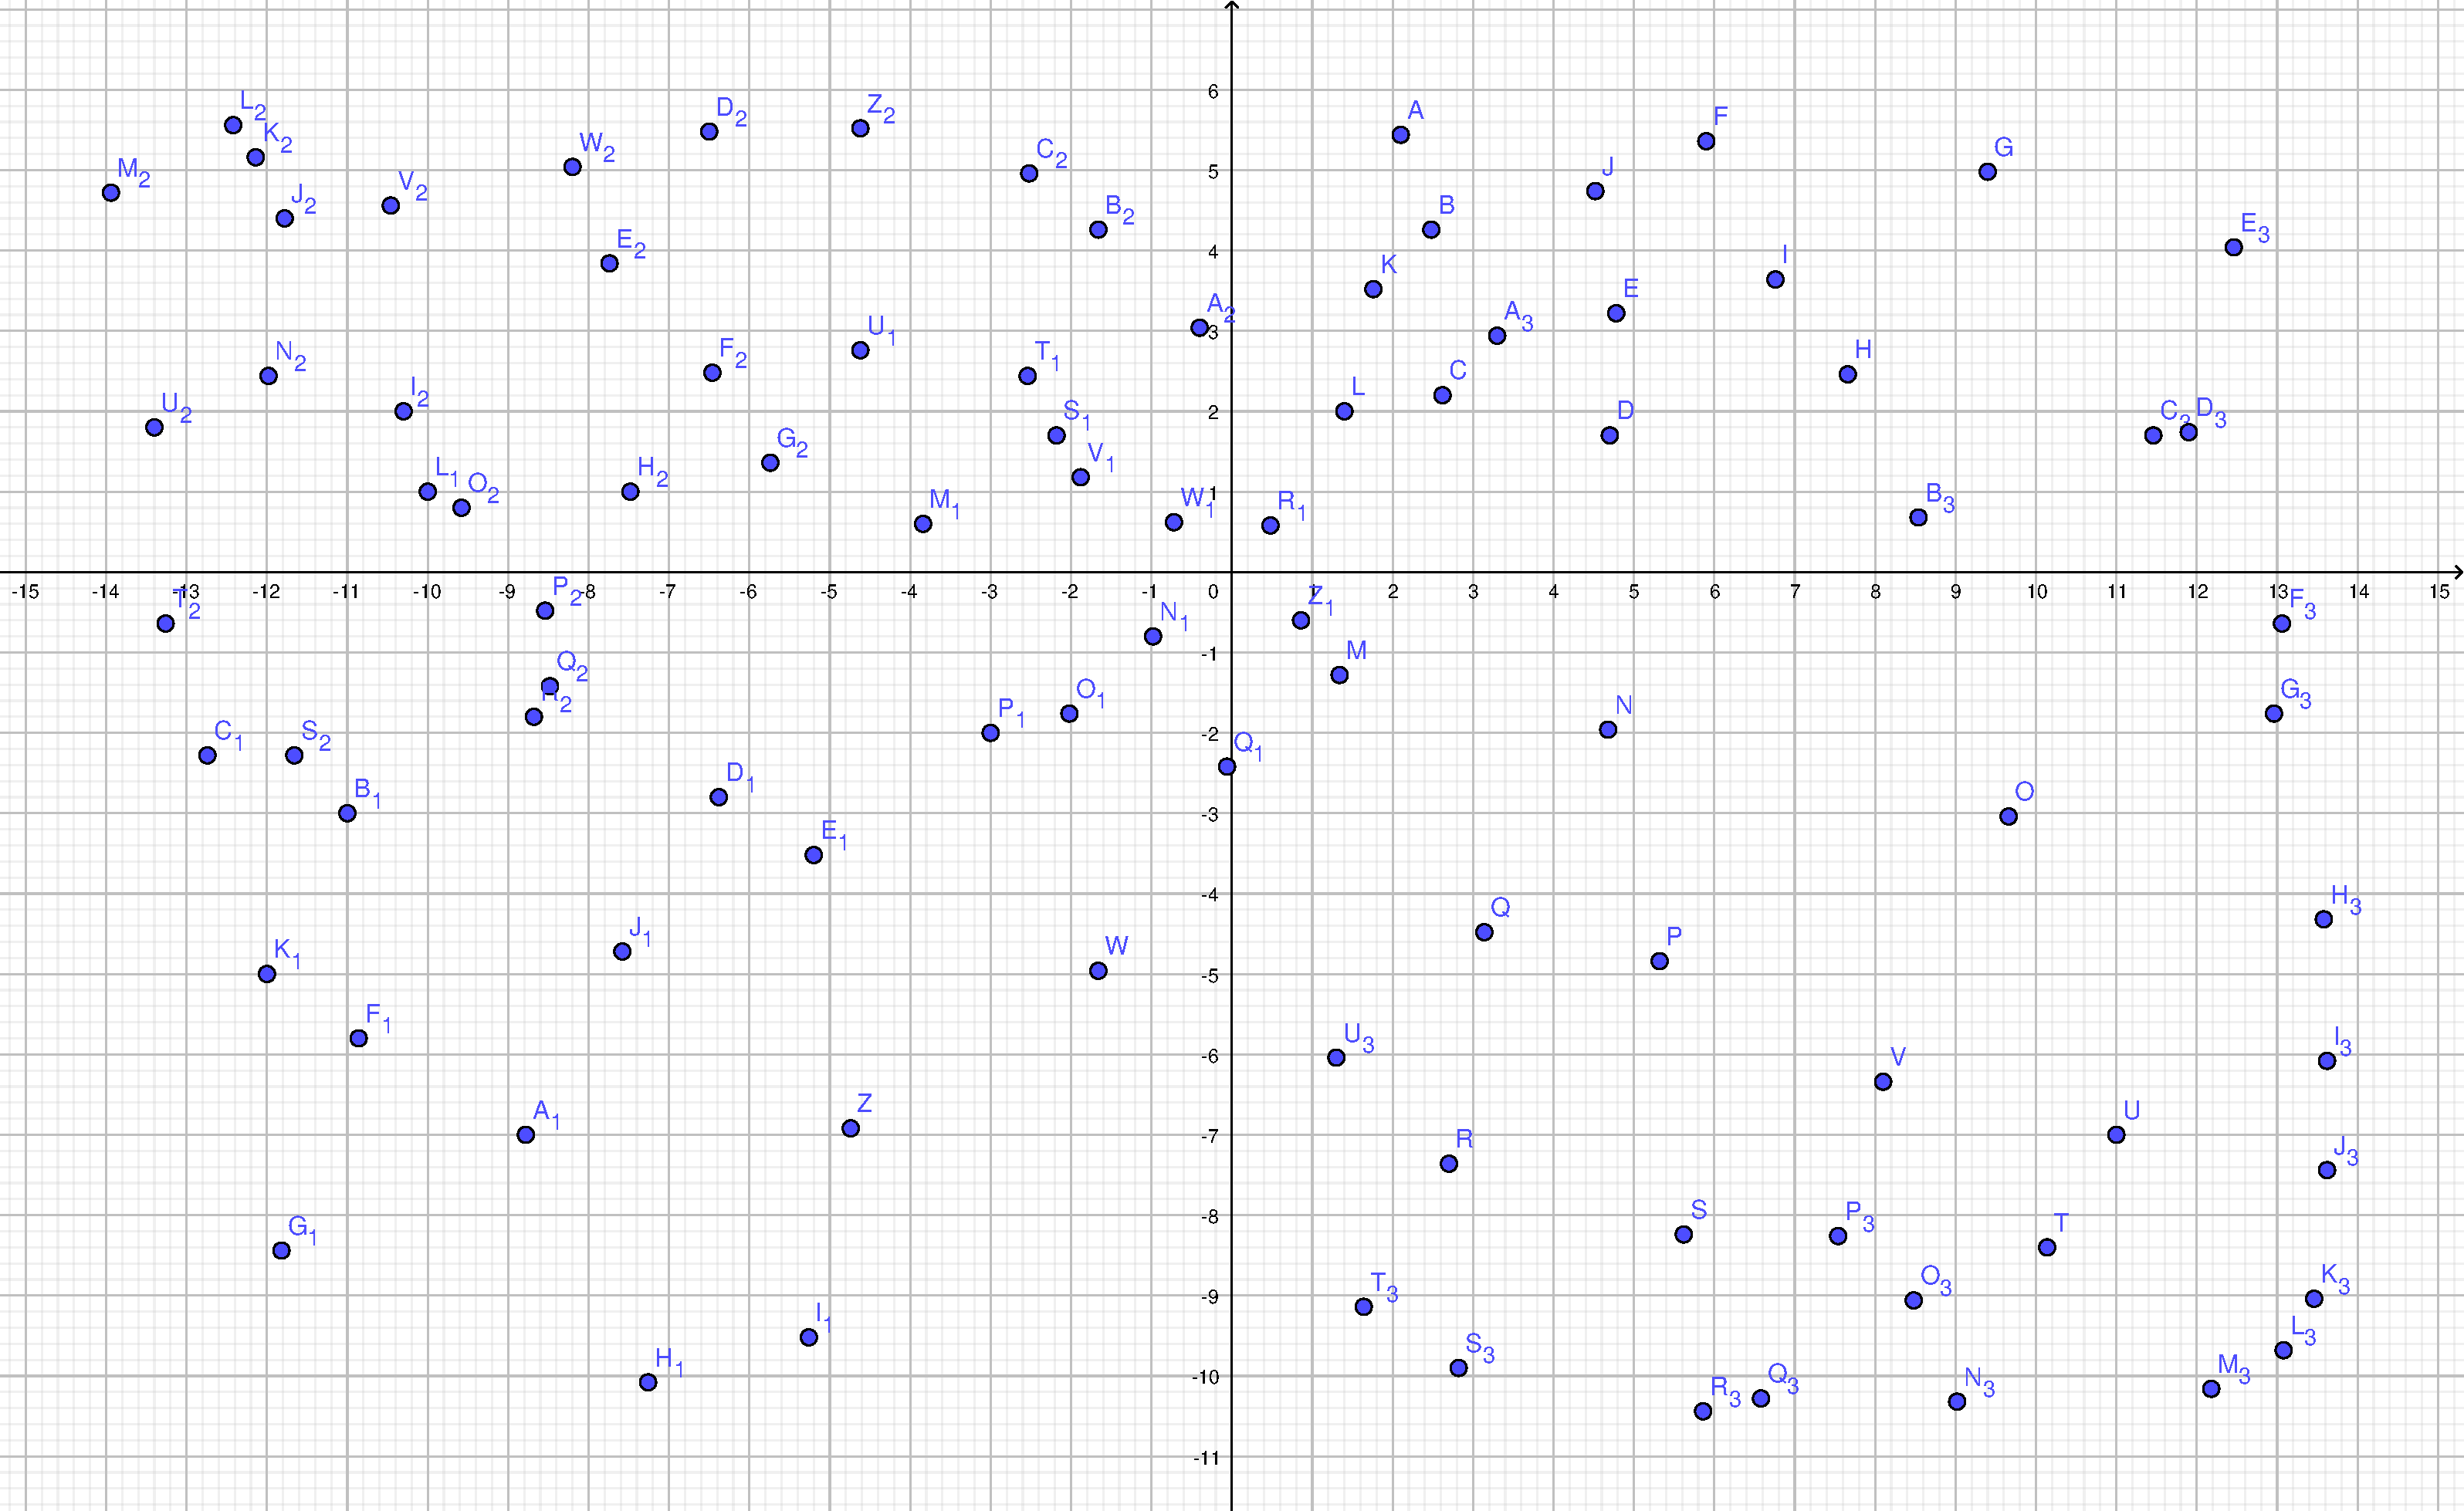
\includegraphics[width=\textwidth]{Gen-i-vyborka.pdf}
\caption{Генеральная совокупность}\label{fig:Gen-sovokup}
\end{figure}

	
Таким образом, процесс предсказания стоимости конкретного объекта происходит в~два~этапа и~на~основе двух принципов:
\begin{enumerate}
	\item формирование выводов о~свойствах всего открытого рынка на~основе изучения выборки "--- \textbf{принцип <<от~частного к~общему>>};
	\item формирование вывода о~стоимости конкретного объекта на~основе установленных свойств открытого рынка, к~которому он~относится "--- \textbf{принцип <<от~общего к~частному>>}.
\end{enumerate}
В~случае необходимости формирования общих выводов о~свойствах рынка достаточно проведение только первой части анализа. 
\section{Типы данных}

\section{Меры центральной тенденции}

\section{Меры изменчивости}

\section{Квантили распределения}

\section{Распределения}

\subsection{Нормальное распределение}

\subsection{Логарифмически нормальное распределение}

\subsection{Равномерное распределение}

\subsection{Экспоненциальное распределение}

\subsection{Нормальное распределение}

\subsection{Распределение Вейбулла}

\subsection{Нормальное распределение}

\subsection{Гамма распределение}

\subsection{Бета распределение}

\subsection{Распределение $\chi ^ 2$~(Распределение Пирсона)}

\subsection{Распределение Стьюдента~(t-распределение)}

\subsection{Распределение Фишера~(F-распределение)}

\subsection{Логистическое распределение}

\subsection{Распределение Парето}

\section{Проверка распределения на~нормальность}

\section{Центральная предельная теорема}

\section{Доверительные интервалы}

\section{Сравнение средних (t-критерий Стьюдента)}

\section{Однофакторный дисперсионный анализ}

\section{ANOVA}

\section{A/B тесты}

\section{Корреляционный анализ}

\subsection{Параметрические методы}

\subsection{Непараметрические методы}

\section{Регрессионный анализ}

\subsection{GLM}

\subsection{Однофакторная линейная регрессия}

\subsection{Множественная регрессия}

\subsection{Логистическая регрессия}

\subsection{Непараметрическая регрессия}







\section{Что~дальше?}
Математическая статистика представляет собой огромную область знаний человека. К~тому~же она~продолжает развиваться. В~данном фрагменте был рассмотрен лишь весьма ограниченный круг вопросов. В~списке источников информации дана некоторая подборка материалов, которые, по~мнению автора, могут быть полезными в~дальнейшем освоении вопросов математической статистики. Поскольку оценщики, как~правило, очень занятые люди, освоение вряд~ли можно ожидать, что~кто-то захочет сразу изучать десятки материалов. В~связи с~этим автор рекомендует ознакомление в~первую очередь со~следующими работами:
	\begin{itemize}
		\item В.\,Cавельев. \emph{Статистика и~котики} ~\cite{Statistika-i-kotiki}. Прекрасная книга для~тех, кто~только начинает погружение в~область математической статистики.
		\item С.\,Бослаф. \emph{Статистика для~всех}~\cite{Statistika-dlya-vsex}. Одна из~лучших книг по~статистике для~тех, кто~не учился по~профилю и~хочет освоить её~методы на~уровне, достаточном для~применения в~профессиональной деятельности.
		\item А.\,Кобзарь. \emph{Прикладная математическая статистика}~\cite{Kobzarq-prikl-mathstat}. Данный материал представляет собой обширное пособие, предназначенное для~тех, кто~уже владеет некоторой базой и~хочет внедрить применение методов математической статистики на~профессиональном уровне.     
	\end{itemize}  

Учиться следует всю~жизнь. Оценочная деятельность трансформируется, и, спустя несколько лет, данное пособие будет казаться детской раскраской. Автор желает читателям непрерывного совершенствования и~становления в~качестве настоящих специалистов в~сфере цифровой оценки XXI~века.

\nocite{Statistika-i-kotiki, Xalqman:Regression-analiz, Baraz:KRA, GOST:Tochnostq-izmerenij-1, GOST:Statmetody, GOST:Statterminy, Stepik:osnovy-statistiki-1, Stepik:osnovy-statistiki-2, Stepik:osnovy-statistiki-3, Teorver-v-uduvolqstvie, CSC:la, CSC:teoriya-grafov, CSC:mathstat-1, CSC:diskt-math, CSC:matan-1, CSC:matan-2, CSC:teorver, CSC:vvedenie-v-matan, Statostika-dlya-gum, Stat-radiosignal, Sprav:mathstat, Math-mod-Kazanczeva, Statistika-dlya-vsex, Veroyatnosty-i-mathstat-Encz, Kobzarq-prikl-mathstat, N-hist, Stat-vyvody-i-svyazi, ITMO:statistika, Drejper-Smith:prikl-regr-analiz, Ajwazyan-prikl-stat, Shixalyyow-Regr-an-par-regr, Biznes-analiz-informaczii:statmetody}
\printbibliography[title=Источники информации]

\end{document}
